\documentclass[10pt,a4paper]{article}
\usepackage{blindtext}
\usepackage{subcaption}
\usepackage{graphicx}
\usepackage{tikz}
\usepackage{amssymb}
\usepackage{caption}
\usepackage{amsmath}
\usepackage{circuitikz}
\usepackage{hyperref}
\usepackage{amssymb}
\usepackage{amsmath}
\usepackage{listings}

\lstset{
    inputencoding=utf8,
    extendedchars=true,
    literate={á}{{\'a}}1 {é}{{\'e}}1 {í}{{\'i}}1 {ó}{{\'o}}1 {ú}{{\'u}}1 {ñ}{{\~n}}1 {Á}{{\'A}}1 {É}{{\'E}}1 {Í}{{\'I}}1 {Ó}{{\'O}}1 {Ú}{{\'U}}1 {Ñ}{{\~N}}1
}
\usepackage[spanish,activeacute,es-tabla]{babel}
\usepackage[utf8]{inputenc}
\usepackage{ifthen}
\usepackage{listings}
\usepackage{dsfont}
\usepackage{subcaption}
\usepackage{amsmath}
\usepackage[strict]{changepage}
\usepackage[top=1cm,bottom=2cm,left=1cm,right=1cm]{geometry}%
\usepackage{color}%
\newcommand{\tocarEspacios}{%
	\addtolength{\leftskip}{3em}%
	\setlength{\parindent}{0em}%
}

% Especificacion de procs

\newcommand{\In}{\textsf{in }}
\newcommand{\Out}{\textsf{out }}
\newcommand{\Inout}{\textsf{inout }}

\newcommand{\encabezadoDeProc}[4]{%
	% Ponemos la palabrita problema en tt
	%  \noindent%
	{\normalfont\bfseries\ttfamily proc}%
	% Ponemos el nombre del problema
	\ %
	{\normalfont\ttfamily #2}%
	\
	% Ponemos los parametros
	(#3)%
	\ifthenelse{\equal{#4}{}}{}{%
		% Por ultimo, va el tipo del resultado
		\ : #4}
}

\newenvironment{proc}[4][res]{%
	
	% El parametro 1 (opcional) es el nombre del resultado
	% El parametro 2 es el nombre del problema
	% El parametro 3 son los parametros
	% El parametro 4 es el tipo del resultado
	% Preambulo del ambiente problema
	% Tenemos que definir los comandos requiere, asegura, modifica y aux
	\newcommand{\requiere}[2][]{%
		{\normalfont\bfseries\ttfamily requiere}%
		\ifthenelse{\equal{##1}{}}{}{\ {\normalfont\ttfamily ##1} :}\ %
		\{\ensuremath{##2}\}%
		{\normalfont\bfseries\,\par}%
	}
	\newcommand{\asegura}[2][]{%
		{\normalfont\bfseries\ttfamily asegura}%
		\ifthenelse{\equal{##1}{}}{}{\ {\normalfont\ttfamily ##1} :}\
		\{\ensuremath{##2}\}%
		{\normalfont\bfseries\,\par}%
	}
	\renewcommand{\aux}[4]{%
		{\normalfont\bfseries\ttfamily aux\ }%
		{\normalfont\ttfamily ##1}%
		\ifthenelse{\equal{##2}{}}{}{\ (##2)}\ : ##3\, = \ensuremath{##4}%
		{\normalfont\bfseries\,;\par}%
	}
	\renewcommand{\pred}[3]{%
		{\normalfont\bfseries\ttfamily pred }%
		{\normalfont\ttfamily ##1}%
		\ifthenelse{\equal{##2}{}}{}{\ (##2) }%
		\{%
		\begin{adjustwidth}{+5em}{}
			\ensuremath{##3}
		\end{adjustwidth}
		\}%
		{\normalfont\bfseries\,\par}%
	}
	
	\newcommand{\res}{#1}
	\vspace{1ex}
	\noindent
	\encabezadoDeProc{#1}{#2}{#3}{#4}
	% Abrimos la llave
	\par%
	\tocarEspacios
}
{
	% Cerramos la llave
	\vspace{1ex}
}

\newcommand{\aux}[4]{%
	{\normalfont\bfseries\ttfamily\noindent aux\ }%
	{\normalfont\ttfamily #1}%
	\ifthenelse{\equal{#2}{}}{}{\ (#2)}\ : #3\, = \ensuremath{#4}%
	{\normalfont\bfseries\,;\par}%
}

\newcommand{\pred}[3]{%
	{\normalfont\bfseries\ttfamily\noindent pred }%
	{\normalfont\ttfamily #1}%
	\ifthenelse{\equal{#2}{}}{}{\ (#2) }%
	\{%
	\begin{adjustwidth}{+2em}{}
		\ensuremath{#3}
	\end{adjustwidth}
	\}%
	{\normalfont\bfseries\,\par}%
}

% Tipos

\newcommand{\nat}{\ensuremath{\mathds{N}}}
\newcommand{\ent}{\ensuremath{\mathds{Z}}}
\newcommand{\float}{\ensuremath{\mathds{R}}}
\newcommand{\bool}{\ensuremath{\mathsf{Bool}}}
\newcommand{\cha}{\ensuremath{\mathsf{Char}}}
\newcommand{\str}{\ensuremath{\mathsf{String}}}

% Logica

\newcommand{\True}{\ensuremath{\mathrm{true}}}
\newcommand{\False}{\ensuremath{\mathrm{false}}}
\newcommand{\Then}{\ensuremath{\rightarrow}}
\newcommand{\Iff}{\ensuremath{\leftrightarrow}}
\newcommand{\implica}{\ensuremath{\longrightarrow}}
\newcommand{\IfThenElse}[3]{\ensuremath{\mathsf{if}\ #1\ \mathsf{then}\ #2\ \mathsf{else}\ #3\ \mathsf{fi}}}
\newcommand{\yLuego}{\land _L}
\newcommand{\oLuego}{\lor _L}
\newcommand{\implicaLuego}{\implica _L}

\newcommand{\cuantificador}[5]{%
	\ensuremath{(#2 #3: #4)\ (%
		\ifthenelse{\equal{#1}{unalinea}}{
			#5
		}{
			$ % exiting math mode
			\begin{adjustwidth}{+2em}{}
				$#5$%
			\end{adjustwidth}%
			$ % entering math mode
		}
		)}
}

\newcommand{\existe}[4][]{%
	\cuantificador{#1}{\exists}{#2}{#3}{#4}
}
\newcommand{\paraTodo}[4][]{%
	\cuantificador{#1}{\forall}{#2}{#3}{#4}
}

%listas

\newcommand{\TLista}[1]{\ensuremath{seq \langle #1\rangle}}
\newcommand{\lvacia}{\ensuremath{[\ ]}}
\newcommand{\lv}{\ensuremath{[\ ]}}
\newcommand{\longitud}[1]{\ensuremath{|#1|}}
\newcommand{\cons}[1]{\ensuremath{\mathsf{addFirst}}(#1)}
\newcommand{\indice}[1]{\ensuremath{\mathsf{indice}}(#1)}
\newcommand{\conc}[1]{\ensuremath{\mathsf{concat}}(#1)}
\newcommand{\cab}[1]{\ensuremath{\mathsf{head}}(#1)}
\newcommand{\cola}[1]{\ensuremath{\mathsf{tail}}(#1)}
\newcommand{\sub}[1]{\ensuremath{\mathsf{subseq}}(#1)}
\newcommand{\en}[1]{\ensuremath{\mathsf{en}}(#1)}
\newcommand{\cuenta}[2]{\mathsf{cuenta}\ensuremath{(#1, #2)}}
\newcommand{\suma}[1]{\mathsf{suma}(#1)}
\newcommand{\twodots}{\ensuremath{\mathrm{..}}}
\newcommand{\masmas}{\ensuremath{++}}
\newcommand{\matriz}[1]{\TLista{\TLista{#1}}}
\newcommand{\seqchar}{\TLista{\cha}}

\renewcommand{\lstlistingname}{Código}
\lstset{% general command to set parameter(s)
	language=Java,
	morekeywords={endif, endwhile, skip},
	basewidth={0.47em,0.40em},
	columns=fixed, fontadjust, resetmargins, xrightmargin=5pt, xleftmargin=15pt,
	flexiblecolumns=false, tabsize=4, breaklines, breakatwhitespace=false, extendedchars=true,
	numbers=left, numberstyle=\tiny, stepnumber=1, numbersep=9pt,
	frame=l, framesep=3pt,
	captionpos=b,
}

\newcommand{\notimplies}{\;\not\!\!\!\implies}
\title{Álgebra I}
\author{Tomás Agustín Hernández}
\date{}

\begin{document}
\maketitle

\begin{figure}[b]
    \centering
    \begin{tikzpicture}[remember picture,overlay]
        \node[anchor=south east, inner sep=0pt, xshift=-1cm, yshift=2cm] at (current page.south east) {
            \begin{minipage}[b]{0.5\textwidth}
                
\includegraphics[width=\linewidth]{logo_uba.jpg}
                \label{fig:bottom}
            \end{minipage}
        };
    \end{tikzpicture}
\end{figure}

\newpage
\section*{Conjuntos}
Los conjuntos almacenan elementos, \textbf{no se consideran repetidos ni tampoco importa el orden}. Responde a la pregunta de $"$¿está el elemento?$"$, esto último quiere decir que no tenemos forma de tomar un elemento sino predicar acerca de si está o no. \\
\textbf{Ej.}: $ A = \{1, 2\}, B = \{2, 1\}$. A y B son considerados iguales, pues no importa el orden sino los elementos que tienen dentro.
\subsection*{Pertenecencia a un Conjunto}
Si consideramos cualquier elemento $x$, decimos que está en un conjunto A si \textbf{x pertenece a A}. \\
La pertenencia de un elemento a un conjunto la denotamos como: $x \in A$ \\
\textbf{Importante}: La relación está dada por $Elemento \ y \ Conjunto$ \\
Véase \hyperref[subsec:pertenecencia_conjuntos]{\underline{ánexo}} para ejemplos más didácticos.
\subsection*{Inclusión a un Conjunto}
Sean A y D conjuntos cualesquiera.
Decimos que D es un subconjunto de A sí y solo sí todos los elementos de D están en A. \\
La inclusión en un conjunto la denotamos como $D \subseteq A$ \\
Es posible leer el símbolo $ \subseteq $ de tres maneras: 
\begin{itemize}
    \item "D es un subconjunto de A"
    \item "D está incluido en A"
    \item "D está contenido en A"
\end{itemize}
Los subconjuntos posibles no salen más que haciendo combinaciones con sus elementos, es decir, agruparlos de diferentes formas. \\
Véase \hyperref[subsec:inclusion_conjuntos]{\underline{ánexo}} para ejemplos más didácticos.
\subsection*{Cardinal de un Conjunto}
Sea A un conjunto, el cardinal de un conjunto indica la cantidad de elementos en el conjunto. \\
Se denota como: $\#A$
\subsection*{Conjunto de Partes}
Se llama A un conjunto, se llama conjunto de partes al conjunto con todos los subconjuntos de A. \\
Se denota como $P(A)$
\begin{itemize}
    \item El elemento vacío $\emptyset \in P(A)$
    \item $A \in P(A)$
    \item $\#P(A) = 2^{\#A}$
\end{itemize}
\subsection*{Cantidad de Subconjuntos posibles dado un Conjunto}
Sea un conjunto A, la cantidad de subconjuntos D para el conjunto A es: $2^{\#A}$
\subsection*{Elemento Vacío}
Se representa con el símbolo de $\emptyset$. El elemento vacío está \textbf{incluido} en todos los conjuntos. \\
\textbf{Importante}: El elemento vacío NO pertenece a todos los conjuntos sino que está incluido en todos.
\subsection*{Cuantificadores}
Nos permiten predicar acerca de los elementos de un conjunto dado. 
\begin{itemize}
    \item $\forall$ x: Para todo x.
    \begin{itemize}
        \item Para que sea verdadero todos deben cumplir la condición dada.
        \item Es falso si existe un caso en que no se cumple.
    \end{itemize}
    \item $\exists$ x: Existe un x
    \begin{itemize}
        \item Para que sea verdadero alcanza con encontrar un caso verdadero.
        \item Es falso si no hay ningun caso que cumpla la condición
    \end{itemize}
\end{itemize}
\textbf{Importante}: El símbolo de $:$ o $/$ significa "tal que" \\
Véase \hyperref[subsec:cuantificadores]{\underline{ánexo}} para ejemplos más didácticos.
\section*{Operaciones entre Conjuntos}
Sean A y B conjuntos cualesquiera. La cantidad de filas que tendrá una tabla de verdad es: \textbf{$2^{cantVariables}$} \\
\textbf{Importante}: Las operaciones entre conjuntos que vamos a ver están relacionadas con la lógica proposicional.
\subsection*{Unión $(A \cup B)$}
Es exactamente igual como en la lógica proposicional. La unión es un $o$ lógico. En el conjunto resultante quedan los elementos de A y B. \\

\begin{table}[h!]
    \centering
    \begin{tabular}{|c | c | c|}
    \hline
    \textbf{A} & \textbf{B} & \textbf{$A \cup B$} \\[0.1cm]
    \hline
    V & V & V \\
    V & F & V \\
    F & V & V \\
    F & F & F \\
    \hline
    \end{tabular}
    \caption{Unión de conjuntos}
\end{table} 
Cada fila se puede generalizar para un x cualquiera en las operaciones lógicas. \\
\textbf{Ej.}: Si $x \in A \land x \in B$ entonces $ x \in A \cup B$ esto claramente nos dice que estamos en el caso de la fila 1. \\
\textbf{Ej.}: Si $x \notin A \land x \in B$ entonces $ x \in A \cup B$ esto claramente nos dice que estamos en el caso de la fila 3.
\subsection*{Intersección $(A \cap B)$}
Es exactamente igual como en la lógica proposicional. La intersección es un $"y"$ lógico. En el conjunto resultante quedan los elementos que están tanto en A y en B.
\begin{table}[h!]
    \centering
    \begin{tabular}{|c | c | c|}
    \hline
    \textbf{A} & \textbf{B} & \textbf{$A \cap B$} \\[0.1cm]
    \hline
    V & V & V \\
    V & F & F \\
    F & V & F \\
    F & F & F \\
    \hline
    \end{tabular}
    \caption{Intersección de conjuntos}
\end{table} \\
Cada fila se puede generalizar para un x cualquiera en las operaciones lógicas. \\
\textbf{Ej.}: Si $x \in A \land x \in B$ entonces $ x \in A \cap B$ esto claramente nos dice que estamos en el caso de la fila 1. \\
\textbf{Ej.}: Si $x \notin A \land x \in B$ entonces $ x \notin A \cap B$ esto claramente nos dice que estamos en el caso de la fila 3.
\subsection*{Complemento $(A \cap B)$}
En la lógica proposicional, el complemento es la negación. Lo que está en un conjunto universal V pero no en el conjunto.
\begin{table}[h!]
    \centering
    \begin{tabular}{|c | c|}
    \hline
    \textbf{A} & \textbf{$\neg A$} \\[0.1cm]
    \hline
    V & F \\
    V & F  \\
    F & V  \\
    F & V \\
    \hline
    \end{tabular}
    \caption{Complemento en Conjuntos}
\end{table} \\
Cada fila se puede generalizar para un x cualquiera en las operaciones lógicas. \\
\textbf{Ej.}: Si $x \in A$ entonces termina siendo $ x \notin A$ esto claramente nos dice que estamos en el caso de la fila 1. \\

Sea $A=\{1, 2\}, B=\{3, 4, 5\}, C=\{8, 9\}, V=\{A, B, C\} \implies A^{c} = \{3, 4, 5, 8, 9\}$ \\
\textbf{Importante}: Nótese que siempre se hace el complemento en base a los elementos que hay en el universo y se excluyen algunos. En este caso, del universo V nos quedamos con los que NO están en A.
\newpage
\subsection*{Diferencia $(A-B )$}
Esta operación es conocida también de la siguiente manera $A\symbol{92}B$.
Es una equivalencia de $A \cap B^{c}$. Representa lo que está en A pero no en B. Si se lo quisiera representar en la tabla de verdad, debe representar la equivalencia.
\begin{table}[h!]
    \centering
    \begin{tabular}{|c | c | c | c|}
    \hline
    \textbf{A} & \textbf{B} & \textbf{$B^{c}$} & \textbf{$A \cap B^{c}$} \\[0.1cm]
    \hline
    V & V & F & F\\
    V & F & V & V\\
    F & V & F & F\\
    F & F & V & F\\
    \hline
    \end{tabular}
    \caption{Diferencia de conjuntos}
\end{table} 
\subsection*{Diferencia Simétrica $(A \triangle B)$}
Equivalente al XOR($\veebar$) u $o$ excluyente en la lógica proposicional. \\
Es una equivalencia de $(A - B) \cup (B - A)$ y $(A\cup B) - (A \cap B)$. Representa lo que está en A o en B pero no en ambos. 
\begin{table}[h!]
    \centering
    \begin{tabular}{|c | c | c | c | c|}
    \hline
    \textbf{A} & \textbf{B} & \textbf{$A \veebar B$} & \textcolor{blue}{$(A - B) \cup (B - A)$} & \textcolor{blue}{$(A\cup B) - (A \cap B)$} \\[0.1cm]
    \hline
    V & V & F & F & F \\
    V & F & V & V & V \\
    F & V & V & V & V \\
    F & F & F & V & V \\
    \hline
    \end{tabular}
    \caption{Diferencia Simétrica en conjuntos}
\end{table} \\
\textbf{Nota}: Las columnas en azul son equivalencias a la operación $\veebar$ y son útiles a la hora de demostrar. \\
\textbf{Ej.}: Si $x \in A \land x \in B$ entonces $ A \veebar B = F$ esto claramente nos dice que estamos en el caso de la fila 1.
\textbf{Ej.}: Si $x \in A \land x \notin B$ entonces $ A \veebar B = V$ esto claramente nos dice que estamos en el caso de la fila 2. \\
\subsection*{Inclusión $(A \subseteq B)$}
Representa el $\implies$ de la lógica proposicional. Recordemos que la inclusión es verdadera si todos los elementos de A están en B siendo A y B conjuntos cualesquiera. \\
Es lo que vamos a utilizar para demostrar, y es importante que se lo entienda bien. 
\begin{table}[h!]
    \centering
    \begin{tabular}{|c | c | c|}
    \hline
    \textbf{A} & \textbf{B} & \textbf{$A \implies B$} \\[0.1cm]
    \hline
    V & V & V \\
    V & F & F \\
    F & V & V \\
    F & F & V \\
    \hline
    \end{tabular}
    \caption{Inclusión de conjuntos}
\end{table} 
\begin{itemize}
    \item El único caso que nos importa es que si el antecedente es verdadero, hay que ver que el consecuente NO sea falso. En las demostraciones asumimos que vale el antecedente y tenemos que ver si hace verdadero al consecuente.
    \item Si no se cumple el antecedente, el consecuente es siempre verdadero.
\end{itemize}
Cada fila se puede generalizar para un x cualquiera en las operaciones lógicas. \\
\textbf{Ej.}: Sea $A = \{1, 2, 3\} \ B = \{10, 40\} \ x = 100$ ¿Se cumple que $ x \in A \implies x \in B$? ¿100 está en A? No, y al ser una implicación si el antecedente no se cumple, queda toda la proposición verdadera. Luego, sí, se cumple que $ x \in A \implies x \in B$. Esto claramente nos dice que estamos en el caso de la fila 3. \\ 
\textbf{Ej.}: Sea $A = \{1, 2, 3\} \ B = \{10, 40\} \ x = 3$ ¿Se cumple que $ x \in A \implies x \in B$? ¿3 está en A? Sí. Entonces esto hace al antecedente verdadero ¿me basta para decir que la proposición es verdadera? No. Primero debo ver qué pasa con el consecuente. ¿Es cierto que 3 está en B? No. Entonces como el antecedente es verdadero y el consecuente es falso, la proposición es falsa. Luego, no, no se cumple que $ x \in A \implies x \in B$. Esto claramente nos dice que estamos en el caso de la fila 2. \\
\textbf{Nota}: Que se entiendan los ejemplos anteriormente mencionados es realmente importante. Se usa en prácticamente todas las demostraciones.\subsection*{Igualdad $(A \iff B)$}
Representa el $\iff$ (sí y solo sí) de la lógica proposicional. Recordemos que la igualdad es verdadera si todos los elementos de A están en B siendo A y B conjuntos cualesquiera. \\
\begin{table}[h!]
    \centering
    \begin{tabular}{|c | c | c|}
    \hline
    \textbf{A} & \textbf{B} & \textbf{$A \iff B$} \\[0.1cm]
    \hline
    V & V & V \\
    V & F & F \\
    F & V & F \\
    F & F & F \\
    \hline
    \end{tabular}
    \caption{Igualdad de conjuntos}
\end{table} 
\begin{itemize}
    \item La manera de demostrar esto es viendo si se cumple que $A \subseteq B \ y \ B \subseteq A$
\end{itemize}
Cada fila se puede generalizar para un x cualquiera en las operaciones lógicas. 
\subsection*{Leyes de De Morgan}
La forma más fácil de verlo es que se distribuye el complemento y se invierte la operación.
\begin{itemize}
    \item $(A \cup B)^{c} = A^{c} \cap B^{c}$
    \item $(A \cap B)^{c} = A^{c} \cup B^{c}$
\end{itemize}
\subsection*{Propiedades de Conjuntos}
\begin{itemize}
    \item Distributiva: $A \cap (B \cup C) = (A \cap B) \cup (A \cap C)$
    \item Conmutatividad: $A \cap B = B \cap A $ Igual para unión
    \item Conjuntos Disjuntos $ A \cap B = \emptyset$
\end{itemize}
TODO: Agregar en Anexo demostración de distributividad.
\subsection*{Producto Cartesiano ($A X B$)}
Sean dos conjuntos A y B cualquiera. El producto cartesiano es el par ordenado (c, d) con $c \in A$ y $d \in B$. \\ 
La cantidad de elementos máxima en un producto cartesiano es = $\#A \ast \#B$. \\
Sí o sí es necesario que el par NO sea nulo, es decir, deben ser elementos válidos. \\
\textbf{Importante}: AXB $\neq$ BXA \\
\textbf{Ej.}: $A = \{1, 2, 3\}, B = \emptyset, AXB = \emptyset$, pues B está vacío. \\
\textbf{Ej.}: $A = \{1, 2, 3\}, B = \{4, 5\}, \#AXB = 6, AXB = \{\{1, 4\}, \{1, 5\}, \{2, 4\}, \{2, 5\}, \{3, 4\}, \{3, 5\} \}$
\section*{Relaciones}
Sean A y B conjuntos. Una relación A en B es un subconjunto cualquiera R de AXB. \\
\textbf{Ej.}: $A = \{1\}, B = \{4, 5\}, AXB=\{\{1, 4\}, \{1, 5\}\}, R = \{(1, 1), (1, 2), (1, 4)\}$ ¿Es R una relación válida de AXB? No, no lo es pues $(1, 1) \in R$ pero $ (1, 1) \notin AXB$
\section*{Relaciones de un conjunto en sí mismo}
Sea A un conjunto cualquiera. Se dice que A está relacionado con A sí y solo sí AXA. \\
Se dice que R es una relación en A cuando $ R \subseteq AXA$ \\
\textbf{Ej.}: $A = \{1, 2, 3\}, AXA=\{\{1, 1\}, \{1, 2\}, \{1, 3\}, \{2, 2\}, \{2, 3\}, \{3, 3\}\}, R = \{\{1, 2\}, \{1, 4\}\}$ ¿Es R una relación válida de AXB? No, no lo es pues $\{1, 4\} \in R$ pero $ \{1, 4\} \notin AXB$ \\
\textbf{Ej.}: $A = \{1, 2, 3\}, AXA=\{\{1, 1\}, \{1, 2\}, \{1, 3\}, \{2, 2\}, \{2, 3\}, \{3, 3\}\}, R = \{(1, 1), (1, 2), (1, 3)\}$ ¿Es R una relación válida de AXB? Sí lo es, pues todos los subconjuntos pertenecientes a R pertenecen a AXA. \\
Veamos ahora \textbf{las propiedades de las relaciones de un conjunto en sí mismo}.
\subsection*{Reflexividad}
Una relación es reflexiva sí y solo sí para todo elemento de A, a está relacionado con A. \\
\textbf{Formalmente}: $ \forall a \in A \implies aRa$ \\
\textbf{Ej.}: $A = \{1, 2, 3\}, AXA=\{\{1, 1\}, \{1, 2\}, \{1, 3\}, \{2, 2\}, \{2, 3\}, \{3, 3\}\}, R = \{(1, 1), (1, 2), (1, 3)\}$ ¿Es R una relación válida de AXB? Sí lo es. ¿Es reflexiva? No, no lo es, pues 2 no está relacionado con 2, ni tampoco 3 con el 3.\\
\textbf{Ej.}: $A = \{1, 2, 3\}, AXA=\{\{1, 1\}, \{1, 2\}, \{1, 3\}, \{2, 2\}, \{2, 3\}, \{3, 3\}\}, R = \{(1, 1), (2, 2), (3, 3), (1, 2)\}$ ¿Es R una relación válida de AXB? Sí lo es. ¿Es reflexiva? Sí, pues para todo elemento a en R, aRa.\\

\textbf{Nota}: Una relación que solamente tiene dentro los elementos aRa es llamada identidad. Considerando el AXA anterior, la relación identidad sería R = $\{(1, 1), (2, 2), (3, 3)\}$  \\
\textbf{Nota}: Si se quisiera buscar un contraejemplo, una buena forma es hallar un elemento que no se relacione con si mismo. 
\subsection*{Simetría}
Sean a, b $\in$ A. Una relación es simétrica sí y solo sí $aRb \implies bRa$. Vulgarmente decimos que si uno está relacionado con el otro, el otro está obligado a estarlo también. \\
\textbf{Formalmente}: $ \forall a, b \in A \ \symbol{92} \ aRb \implies bRa$ \\
\textbf{Ej.}: $R = \{(1, 2), (3, 1)\}$, no es simétrica pues sucede que $1R2$ pero 2 no está relacionado con 1. \\
\textbf{Ej.}: $R = \{(1, 2), (2, 1)\}$, es simétrica pues para todo elemento relacionado, se relacionan conjuntamente. \\
\textbf{Ej.}: $R = \{(1, 1)\}$, es simétrica, pues no existe ninguna relación entre elementos diferentes. Por lo tanto, el antecedente es falso, luego la proposición ($aRb \implies bRa$) es verdadera \\

\textbf{Nota}: Como es una implicación, si el antecedente es falso (no hay ningún elemento, o no existe relación entre ellos) entonces es simétrica.  \\
\textbf{Nota}: Si se quisiera buscar un contraejemplo, una buena forma es buscar simplemente un elemento que se conecte con otro, pero no al revés.
\subsection*{Antisimétrica}
Sean a, b $\in$ A. Una relación es antisimétrica sí y solo sí $aRb \land bRa \implies A = B$. Vulgarmente decimos que si ambos están relacionados, entonces es porque son iguales. \\
\textbf{Formalmente}: $ \forall a, b \in A \ \symbol{92} \ aRb \land bRa \implies a=b$ \\
\textbf{Ej.}: $R = \{(1, 2), (2, 1)\}$, no es antisimétrica pues 1 se relaciona con 2, y 2 se relaciona con 1 pero $1 \neq 2$ \\
\textbf{Ej.}: $R = \{(1, 1), (2, 2)\}$, es antisimétrica pues 1 se relaciona con 1, 2 se relaciona con dos y son los mismos elementos. \\

\textbf{Nota}: Si se quisiera buscar un contraejemplo, una buena forma es buscar un conjunto que la haga simétrica considerando la relación entre elementos diferentes.
\subsection*{Transitividad}
Sean a, b $\in$ A. Una relación es transitiva sí y solo sí $aRb \land bRc \implies aRc$. Vulgarmente decimos que si a me conecta con la calle b, y b con la calle c, entonces a me lleva a c. \\
\textbf{Formalmente}: $ \forall a, b \in A \ \symbol{92} \ aRb \land bRc \implies aRc$ \\
\textbf{Ej.}: $R = \{(1, 2), (2, 3), (1, 3) \}$, es transitiva pues como 1 me conecta con 2, y 2 se conecta con 3, entonces desde 1 puedo llegar a 3. \\
\textbf{Nota}: Si se quisiera buscar un contraejemplo, una buena forma es buscar un a que esté relacionado con un b, y ese b esté relacionado con un c pero a no esté relacionado con c. Básicamente, sería hacer que se cumpla el antecedente pero no el consecuente.
\subsection*{Relación Identidad}
Dado un conjunto A relacionado y en sí mismo AXA. Una relación R es identidad sí y solo sí todos los elementos de R cumplen la forma de (a, a). \\
\textbf{Ej.}: $R = \{(1, 1), (2, 2), (3, 3)\}$. Es identidad. \\
\textbf{Ej.}: $R = \{(1, 2), (3, 3) \}$. No es identidad pues $1 \neq 2$.
\subsection*{Relación Total}
Dado un conjunto A. Una relación R es total cuando R = AXA.
\subsection*{Clases de Equivalencia}
\label{subsec:clases_equivalencia}
Sea A un conjunto y una relación de equivalencia en A. \\
Para cada $x \in A$, la clase de equivalencia de x es el conjunto: $\bar{x} = [x] = \{y \in A \ \symbol{92} \ yRx\} \subseteq A$. Vulgarmente hablando, es el conjunto de los elementos con los que se relaciona x.
\textbf{Ej.}: $ R = \{(1,1), (1, 2), (2, 1), (3, 1), (1, 3), (4, 5), (5, 4), (6, 6)\}$
\begin{itemize}
    \item $[1] = [2] = [3] =  \{1, 2, 3\}$
    \item $[4] = [5] = \{4, 5\}$
    \item $[6] = \{6\}$
\end{itemize}
\textbf{Propiedad fundamental}: O Sucede $ \bar{x} = \bar{y}$ o sucede $\bar{x} \cap \bar{y} = \emptyset $ pero no ambas a la vez. \\
TODO: Añadir los ejemplos que hice en la tablet al anexo.
\subsection*{Representante de clase}
Cualquier elemento de una clase de equivalencia representa a su clase. 
En la sección de \hyperref[subsec:clases_equivalencia]{\underline{\textbf{Clases de Equivalencia}}} cada clase $[x]$ es representada por x. \\
\section*{Funciones}
Una función $A \leftarrow B$ es una relación $ f \subseteq AXB$ entre A y B que satisface: 
\begin{itemize}
    \item $\forall a \in A, \exists! \ b \in B \ / \ (a, b) \in f$. Si a la función le mando un a, me devuelve siempre el mismo b (no existe más de un b para un mismo a).
\end{itemize}
En las funciones, el valor de b está determinado por a, es decir, $b = f(a)$. \\
Para ser función, se debe cumplir \textbf{existencia ($\forall a \in A$)} y \textbf{unicidad ($\exists! \ b $)}. \\
\textbf{Dominio}: Son los valores los cuales podemos observar y enviar para que el codominio nos arroje un resultado. \\
\textbf{Codominio}: Son el resultado para un x dado que proviene del Dominio. \\
Veamos ahora \textbf{los distintos tipos de funciones}.
\subsection*{Función Inyectiva}
Sean x, y x'. Si sucede que f(x) = f(x') entonces x = x'. \\
Vulgarmente hablando, no existen dos x diferentes tal que el valor que arroja la imagen es el mismo.
\[\begin{minipage}[b]{0.9\textwidth}
    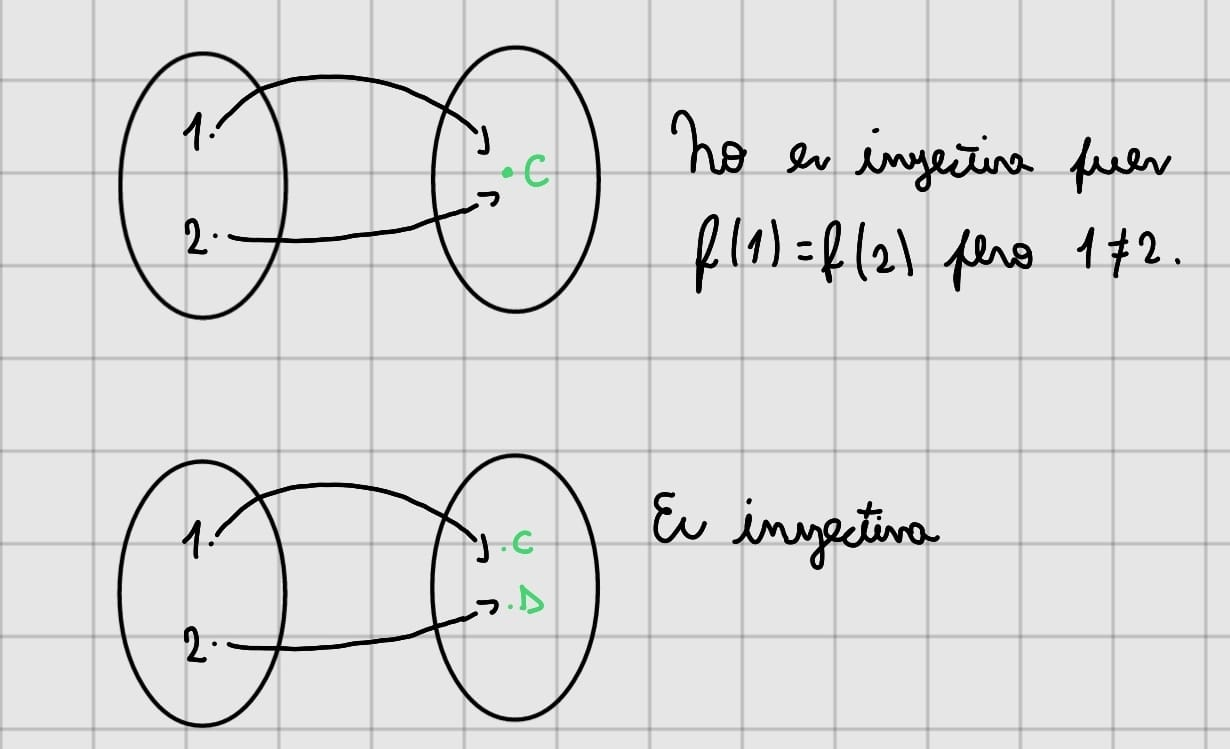
\includegraphics[width=\linewidth]{assets/def_inyectiva.jpg}
    \label{fig:def_inyectiva}
\end{minipage}\]
\subsection*{Función Sobreyectiva}
Sea $f:A \rightarrow B$. Una función es sobreyectiva si $ \forall b \in B, \exists a \ / \ f(a) = b$. \\
Vulgarmente hablando, todos los posibles valores del codominio corresponden con algún valor del dominio.
\[\begin{minipage}[b]{0.9\textwidth}
    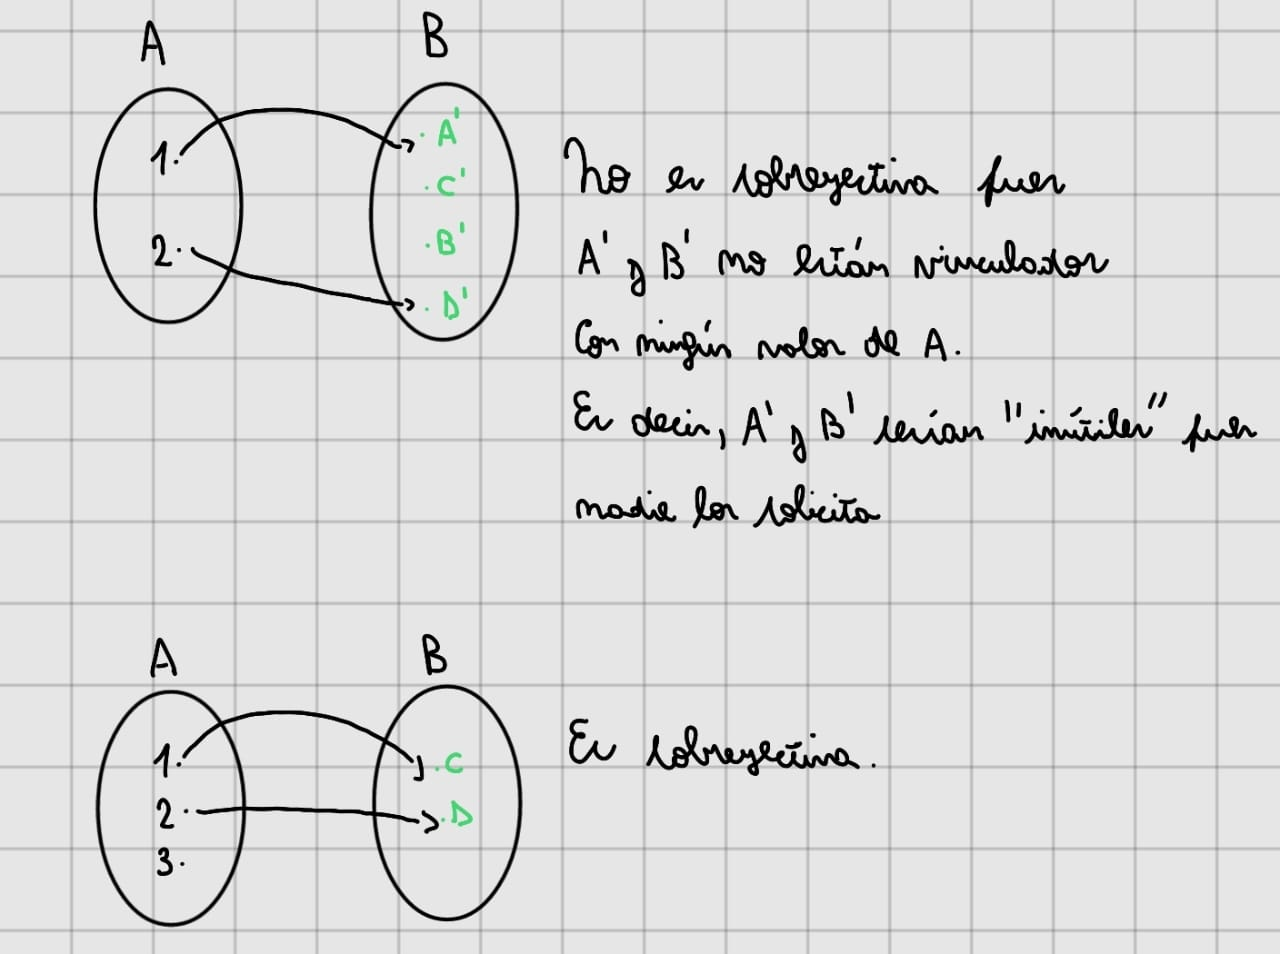
\includegraphics[width=\linewidth]{assets/def_sobreyectiva.jpg}
    \label{fig:def_sobreyectiva}
\end{minipage}\]
\subsection*{Función Biyectiva}
Si es Inyectiva y Sobreyectiva a la vez, entonces es biyectiva.
\[\begin{minipage}[b]{0.9\textwidth}
    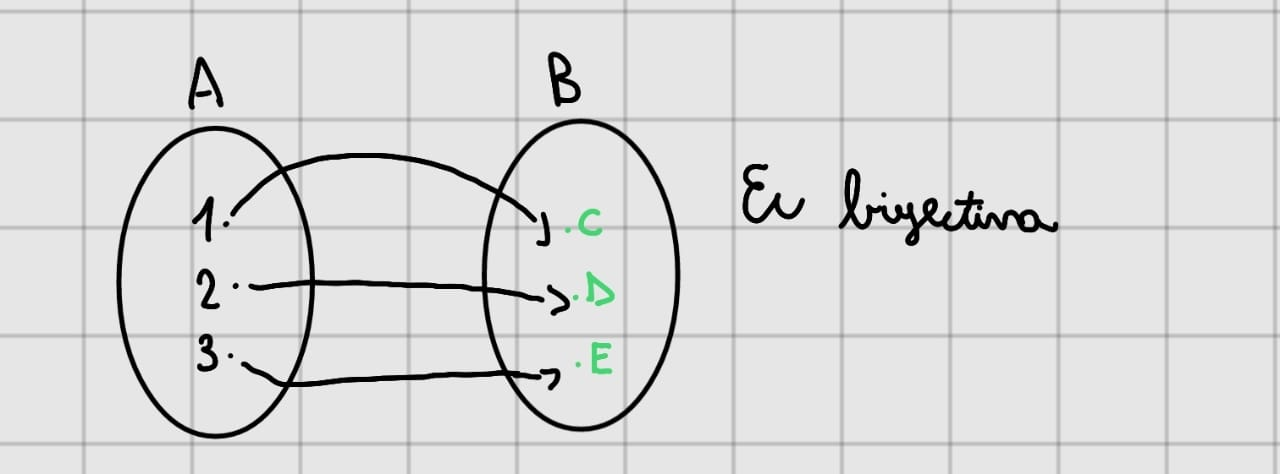
\includegraphics[width=\linewidth]{assets/def_biyectiva.jpg}
    \label{fig:def_biyectiva}
\end{minipage}\]
TODO: Añadir los ejemplos que hice en la tablet al anexo.
\subsection*{Composición de Funciones}
Sean las relaciones $R = AX\bar{B}$ y $S = \bar{B}XA$. \\
La composición de R y S es la relación de A a C dada por: 
$ SoR = \{(a, c) \in AXC, \ \exists b / (a, b) \in R \land (b, c) \in S\}$
\[\begin{minipage}[b]{0.9\textwidth}
    \includegraphics[width=\linewidth]{assets/composicion_funciones.png}
    \label{fig:composicion_funciones}
\end{minipage}\]
\textbf{Ej.}: $f:A\rightarrow B \ g:B\rightarrow C \ gof: A\rightarrow C$ \\
\textbf{Nota}: gof = g es el codominio y f el dominio. \\
Propiedades: 
\begin{itemize}
    \item Si $f:A\rightarrow B \land g:B\rightarrow C$ son funciones entonces $gof$ también.
    \item $I_{A}: A \rightarrow A$
    \item $I_{A} \ o \ f = f$ 
\end{itemize}
\subsection*{Función Inversible}
Si $f:A\rightarrow B$ su inversa es $g:B\rightarrow A$ y la denotamos como $f^{-1}$. \\
Decimos que una función f es inversible si es biyectiva y hay una función g tal que:
\begin{itemize}
    \item $fog = I_{B}$
    \item $gof = I_{A}$
\end{itemize}
Y en ese caso decimos que g es inversa de f. \\
\section*{Naturales - Inducción}
\subsection*{Números Naturales}
Son un conjunto infinito. \\
Algunas propiedades:
\begin{itemize}
    \item Conmutatividad: $ m+n = n+m$
    \item Asociatividad: $(m+n)+k = m+(n+k)$ y $ (m\ast n)\ast k = m\ast (n\ast k)$
    \item Distributividad: $m(n+k) = mn + mk$
\end{itemize}
\subsection*{Sumatoria}
Permite indicar claramente cuantas veces hay que sumar algo dado: $ a_{1} + a_{2} + a_{3} + ... + a_{n-1} + a_{n} \equiv \sum_{i=1}^{n}{a_{i}}$ \\
Los límites superior e inferior de la sumatoria son \textbf{inclusivos} por lo tanto, el último caso es $i=n$.
Algunos casos bastante comunes:
\begin{itemize}
    \item Sumar 1 n veces: \[\sum_{i=0}^{n}{1} = n\]
    \item Sumar los n términos: \[\sum_{i=0}^{n}{i} = \frac{n(n+1)}{2}\]
\end{itemize}
\textbf{Importante}: Es posible manejar los términos de la sumatoria manipulando los límites. \\
Ej.: \[\sum_{i=\textbf{0}}^{\textbf{n+1}}{i} \equiv \sum_{\textbf{i=1}}^{\textbf{n}}{i} \] 
Nótese que en ambos se hace la misma cantidad de operaciones aunque hayamos quitado el n+1 y empezar la sumatoria desde 1 e ir hasta n, pero en el caso de la sumatoria de la derecha podemos aplicar un algoritmo conocido. \\
\textbf{Propiedades de la Sumatoria}: 
\begin{itemize}
    \item \textbf{Juntar sumatorias}: $\sum_{k=1}^{n}{a_{k}} + \sum_{k=1}^{n}{b_{k}}  \equiv \sum_{k=1}^{n}{a_{k} + b_{k}} $, como ambos van desde k = 1 hasta un n dado y los términos van en sincronía con k podemos juntarlos en una sola sumatoria.
    \item \textbf{Distribución denominador en suma}: $\sum_{k=1}^{n}{\frac{a+b+c}{d+c}} \equiv \sum_{k=1}^{n}{\frac{a}{d+c} + \frac{b}{d+c} + \frac{c}{d+c}}$
    \item \textbf{Quitar constante}: $\sum_{k=1}^{n}{c \ast a_{k}} \equiv c \ast \sum_{k=1}^{n}{a_{k}}$
    \item \textbf{Extraer términos}: $\sum_{k=1}^{2^{n+1}}{k^{2}} \equiv \sum_{k=1}^{2^{n} \ast 2}{k^{2}} \equiv \sum_{k=1}^{2^{n}}{k^{2}} + \sum_{k=2^{n}+1}^{2^{n+1}}{k^{2}} $, útil en inducción, lo veremos más adelante.
    \item \textbf{Agregar término}: $\sum_{i=k+1}^{n}{2i+1} \equiv (\sum_{i=k}^{n}{2i+1}) - 2(k+1)+1$, útil en inducción, lo que hacemos es que al agregar un término, se lo restamos en la suma final pues solo agregamos ese término por comodidad pero no se nos pedía en la suma original.
\end{itemize}
\subsection*{Suma de Gauss}
Un poco de contexto: ¿como hacemos para sumar los n números naturales? utilizamos la suma de gauss. \\
Es súper útil conocer esto porque he visto lugares donde suman los primeros n elementos utilizando un for. \\
\[\sum_{i=1}^{n}{i} = \frac{n(n+1)}{2} \] 
\textbf{Importante}: en la materia se utiliza todo el tiempo, por lo tanto no se recomienda memorizarla pero sí entenderla.
\subsection*{Serie Geométrica}
Un poco de contexto: ¿cómo hacemos para sumar los n términos que solo cambia el valor de la potencia? utilizamos la serie geométrica. \\
La serie geométrica se separa en dos casos, cuando $q=1$ y cuando $q\neq 1$
\[Q = \sum_{i=0}^{n}{q^{i}} = \left\{ \begin{array}{lcc} \frac{q^{n+1}-1}{q-1} & si & q \neq 1 \\ \\ n+1 & si & q = 1 \end{array} \right.\]
\subsection*{Productoria}
Mismo que la sumatoria pero de multiplicación: $ a_{1} \ast a_{2} \ast a_{3} \ast ... \ast a_{n-1} \ast a_{n} \equiv \prod_{i=1}^{n}{a_{i}}$ \\
\textbf{Importante}: en la materia se utiliza todo el tiempo, por lo tanto no se recomienda memorizarla pero sí entenderla. \\
Algunos casos bastante comunes:
\begin{itemize}
    \item Multiplicar los n términos: \[\prod_{i=1}^{n}{i} = n!\]
    \item Exponenciación: \[\prod_{i=1}^{n}{c} = c^{n}\]
\end{itemize}
\textbf{Importante}: Al igual que en la sumatoria, podemos manipular los límites superior e inferior. \\
\textbf{Propiedades de la Productoria}: 
\begin{itemize}
    \item \textbf{Juntar productorias}: $\prod_{k=1}^{n}{a_{k}} + \prod_{k=1}^{n}{b_{k}}  \equiv \prod_{k=1}^{n}{a_{k} + b_{k}} $, como ambos van desde k = 1 hasta un n dado y los términos van en sincronía con k podemos juntarlos en una sola productoria.
    \item \textbf{Quitar constante}: $\prod_{k=1}^{n}{c \ast a_{k}} \equiv c^{n} \ast \prod_{k=1}^{n}{a_{k}}$
    \item \textbf{Factor común}: $\prod_{k=1}^{n}{\alpha \ast a_{i} \ast b_{i}} \equiv  \alpha^{n} \ast \prod_{k=1}^{n}{a_{i} \ast b_{i}} \equiv \alpha^{n} \ast \prod_{k=1}^{n}{a_{i}} \ast \prod_{k=1}^{n}{b_{i}} $
    \item \textbf{Agregar término}: $\prod_{i=k+1}^{n}{2i+1} \equiv (\prod_{i=k}^{n}{2i+1}) \ast \frac{1}{2(k+1)+1}$, útil en inducción, lo que hacemos es que al agregar un término. Como acá es una productoria lo que hacemos es "dividir" en vez de restar, que a su vez dividir es multiplicar por 1/algo.
\end{itemize}
\section*{Anexo}
\subsection*{Pertenencia en Conjuntos}
\label{subsec:pertenecencia_conjuntos}
Sea A el conjunto: $\{1, 2, \{C, B\}, F, \{10, 15\}\}$
\begin{itemize}
    \item $ 1 \in A, 2 \in A, F \in A $
    \item $ C \notin A, B \notin A $
    \item $  \{C, B\}, \{10, 15\} \in A $
\end{itemize}
¿Por qué $C \notin A$? Pues C no es un elemento de A.\\ Notar que C es parte del elemento $\{C, B\}$ en A, pero C no es un elemento independiente.
\subsection*{Inclusión en Conjuntos}
\label{subsec:inclusion_conjuntos}
\textbf{Ex. 1}: Sea $A = \{1, 2, 3\} \ y \ D = \{1, 3\}$. ¿Es D un subconjunto de A? \\
Sí, lo es pues $1 \in A$ y $ 3 \in A$ \\
\textbf{Ex. 2}: Sea $A = \{1, \{1, 4\}, 3, 10\}$
\begin{itemize}
    \item $ \{1, 4\} \nsubseteq A $ pues no existen 1 y 4 como elementos en A
    \item $ \{1, 4\} \in A $ pues $\{1, 4\} es un elemento de A$
    \item $\{1, 3\} \subseteq A$ pues $ 1 \in A, 3 \in A$, lo mismo sucede con $ \{1, 10\} \ o \ \{3, 10\}$
\end{itemize}
\subsection*{Cuantificadores}
\label{subsec:cuantificadores}
\textbf{Ex. 1}: $A = \{2, 4, 6, 8\}$ \\
Algunos ejemplos utilizando cuantificadores 
\begin{itemize}
    \item $\forall x \in A \ \symbol{92} \ x \% 2 = 0$ (Todos pares en A)
    \item $\neg \ \exists x \in A \ \symbol{92} \ x \% 2 \neq 0$ (No existe ningún impar en A) 
    \item $ \exists x \in A \ \symbol{92} x = 4$ (Existe un elemento en A que es exactamente 4)
\end{itemize}

\end{document} 

